%second chapter of your thesis
\chapter{Methode en uitwerking}
\label{mRef}
In dit hoofdstuk bespreken we de gebruikte werkwijzen, technieken en materialen. We beginnen met een algemeen blokschema van het te ontwerpen systeem is te vinden in secite \ref{MRefWeS}. Voor ons systeem hebben we ook een camera nodig. Welk type van camera we gebruiken en de plaatsing van deze camera bespreken we in sectie \ref{MRefIRC}. Vervolgens gaan we aan de hand van dit blokschema de manieren bespreken waarmee we de gedragsanalyse geconstrueerd hebben, dit gebeurt in sectie \ref{MRefMGA}. Na de bespreking van de gedragsanalyse, bespreken we de overige methoden van onze code en waarvoor ze gebruikt kunnen worden, dit gebeurd in sectie \ref{MrefOvM}.

\section{Werkingsschema}
\label{MRefWeS}
\begin{figure}[hbp]
	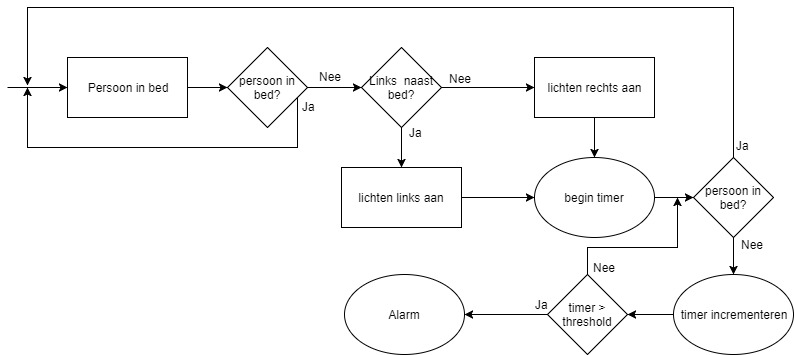
\includegraphics[scale=0.5]{HoogNiveauBlokDiagram}
	\caption{Werkingsschema op hoog niveau}
	\label{imgWeS}
\end{figure}
Dit onderzoek heeft als doel het ontwikkelen van een visiesysteem dat kan detecteren langs welke zijde een pati\"ent uit bed stappt en kan meten hoelang de pati\"ent wegblijft. Als mogelijke uitbereiding kunnen we ook val detectie toevoegen. In figuur \ref{imgWeS} is het werkingsschema op hoog niveau te zien.
We beginnen links bij persoon in bed. We gaan er vanuit dat er een persoon in het bed ligt.  Vervolgens gaan we testen of er delen van het lichaam zich uit het bed bevinden, op welke manier we dit doen, wordt later besproken in sectie \ref{mRefOGA}. Indien er een persoon in het bed gevonden wordt, blijven we deze test herhalen. Is er geen persoon in het bed gedetecteerd, gaan we kijken naar welke zijde. Vanaf het moment dat de persoon het bed heeft verlaten, wordt er een timer gestart. Vervolgens gaan we terug kijken of er een persoon in he bed is. Als er een persoon is, dan gaan we terug naar de startpositie. Als er geen persoon in het bed is, wordt de waarde van de timer ge\"incrementeerd. Daarna gaan we de waarde van de timer vergelijken met een threshold. Is de waarde van de teller groter dan de threshold, dan gaat er een alarm afgaan, deze persoon is te lang uit het bed. Indien de waarde van de timer kleiner is dan de threshold, gaan we terug nazien of er een persoon in het bed is.  De waarde van de threshold kan in het programma aangepast worden als het toilet zich ver van het bed bevindt.  Als de persoon terug in het beeld komt, stopt de teller en bevinden we ons weer in de eerste toestand.

\section{IR camera}
\label{MRefIRC}
Voor de uitwerking van ons project maken we gebruik van een infrarood camera. Deze hebben we eerder al besproken in onze literatuurstudie \ref{refIRC}. We gebruiken deze camera omdat deze ter beschikking werd gesteld door de school en dit ons ook een logische keuze leek. Dit omdat de persoon door de infraroodbeelden al minder snel herkenbaar zijn, op de beelden, wat een zeer belangrijk deel is van de specificaties. Verder is dit in verhouding met de andere besproken types van camera's in de literatuurstudie\ref{refTVC}, een goedkope camera. Verder is in onze toepassing het niet nodig om een gedetailleerd beeld van de pati\"ent te verkrijgen. Hierdoor is de constructie van IP en PTZ camera's hier niet van toepassing. Andere types van camera zouden ook kunnen gebruikt worden. Maar dit onderzoek, is door bovenvermelde redenenen, niet door ons gedaan. We bespreken de gebruikte camara, namelijk die Seek Thermal Compact in sectie \ref{mRefSTh}. Voor de plaatsing van onze camera hebben we een aantal berekeningen gedaan. Dit om te zien waar en op welke hoogte onze camera het beste geplaatst wordt. Deze berekeningen zijn te vinden in sectie \ref{mRefSTP}.

\subsection{Seek Thermal Compact}
\label{mRefSTh}

\begin{figure}[hbp]
	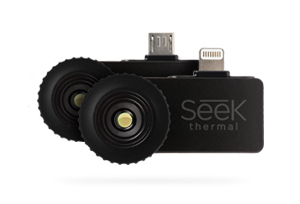
\includegraphics[scale=0.75]{SeekThermalCompac}
	\caption{Image of Seek Thermal Compact}
	\label{imgSTC}
\end{figure}
Dit is een zeer kleine camera die bedoeld is om te gebruiken met een Android smartphone of met een IPhone. Een afbeelding van de camera is terug te vinden in figuur \ref{imgSTC} \cite{bibImgSTC}. Wij hebben gebruik gemaakt van de versie die normaal op Android gestuurde systemen werkt. Om deze camera te kunnen gebruiken op een computer, hebben we gebruik gemaakt van code die ons beschikbaar is gesteld via Eavise \cite{bibSTC}. Via deze code kunnen we van de camera binnen halen en bekijken. Deze camera is gebruikt om alle testbeelden te maken tijdens de experimenten die besproken worden in hoofdstuk \ref{ERef}. Hieronder bespreken we de specificaties van de Seek Thermal Compact voor gebruik op Android toestellen \cite{bibImgSTC}: 
\begin{itemize}
	\item $\mu$USB Thermal Camera for Android devices
	\item Werkt met de meeste Android toestellen die werken met 4.3 of hoger. (Op de website, \url{http://www.thermal.com/products/compact/} is een lijst met compatibele modellen te vinden. 
	\item 206 * 156 Thermal Sensor
	\item 12 $\mu$ Pixel Pitch
	\item Vanadium Oxide Microbolometer
	\item Chalocogeninde Lens
	\item $36^{\circ}$ zicht
	\item Magnesium behuizing
	\item Lange golf infrarood 7.2 - 13 $\mu$m
	\item  spectrum van -40 tot 330 $^{\circ}$c
	\item 9Hz
	\item Bevat een waterdichte cover
	\item Model: UW-AAA
\end{itemize}
Een nadeel van deze camera is dat hij via een $\mu$USB connectie met de computer verbonden moet worden. Hierdoor mag de camera niet te ver staan van de computer waarop het programma met de gedragsanalyse draait, of er moet onderzoek gedaan worden naar een mogelijkheid om de beelden draadloos door te sturen.

\subsection {Plaatsing van de camera}
\label{mRefSTP}
Er zijn verschillende manieren, om de camera te plaatsen. Maar aangezien we het bed in de code moeten kunnen detecteren, willen we dat de positie van het bed hetzelfde blijft ten opzichte van de camera. Hierdoor moeten we een gebruik maken van een statische opstelling. Dit kunnen we doen door de camera via een constructie aan het bed te bevestigen. Een andere manier om een statische opstelling te verkrijgen, is door de camera te bevestigen aan het plafond of \'e\'en van de muren van de kamer.  We weten de openingshoek van de camera. Dankzij deze kunnen we de nodige hoogte van de camera berekenen. We nemen de lengte van het bed (2m) als de bepalende factor voor de hoogte. De camera mag altijd hoger bevestigd worden, zo gaat er meer van de omgeving waargenomen worden. 

\subsubsection{Camera recht boven hoofdeinde}
De eerste berekening die we doen, is een situatie waar de camera recht boven het hoofdeinde geplaatst is. Deze kan zowel via aan constructie aan het bed gemonteerd worden als rechtstreeks aan het plafond. De camera hangt in het midden van de breedte van het bed. Op afbeelding \ref{imgCBB} is een schets van de situatie te zien. 
\begin{figure}[hbp]
	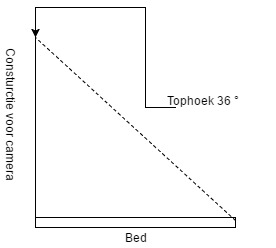
\includegraphics[scale=0.7]{CamBovenBed}
	\caption{Schets van camera recht boven bed}
	\label{imgCBB}
\end{figure}
De berekening van de hoogte is in dit geval heel eenvoudig. Het gaat hier over een rechthoekige driehoek. We kunnen her gebruikt maken van de goniometrische regels voor rechthoekige driehoeken.
\begin{displaymath}
tan(\alpha) =\frac{o}{x}
\end{displaymath}
\begin{displaymath}
tan(36^\circ) = \frac{2}{x}
\Rightarrow x = \frac{2}{tan(36 ^\circ)} = 2,75
\end{displaymath}
met
\begin{itemize}
	\item $\alpha$ is de openingshoek van de camera in uitgedrukt graden
	\item o is de lengte van het bed uitgedrukt in meter
	\item x is de gevraagde hoogte in meter
\end{itemize}
Uit de berekeningen blijkt dat de camera 2,75 meter boven het bed moet hangen. Dit is onmogelijk, omdat de gemiddelde kamer ongeveer een 2,5 meter hoog is. Hierdoor zullen we de camera moeten hangen op een andere locaties. Hieronder volgen de berekeningen voor de situatie waarbij de camera niet recht boven het hoofdeinde hangt.

\subsubsection{Camera niet recht boven hoofdeinde}
\begin{figure}[hbp]
	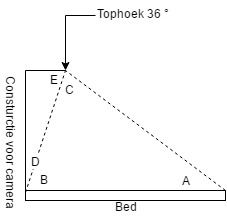
\includegraphics[scale=0.7]{CameraNietRechtBoven}
	\caption{Schets van camera niet recht boven bed}
	\label{imgCNRBB}
\end{figure}
Nadat we uit de voorgaande berekening hebben kunnen besluiten dat het onmogelijk is het bed volledig op het frame te krijgen als we de camera recht boven het hoofdeinde hangen. Gaan we de nodige hoogte bepalen als de camera boven het bed komt te hangen, maar niet recht boven het hoofdeinde. figuur \ref{imgCNRBB} geeft een schets weer van de situatie. De camera hang in het midden van de breedte van het bed. De drukletters in de figuur \ref{imgCNRBB} zijn de verschillende hoeken. Deze worden ook in de berekening gebruikt .Door te rekenen met hoeken in driehoeken en het gebruik van de sinusregels voor willekeurige- en rechthoekige driehoeken, kunnen we de gezochte hoogte berekenen. Alle hoeken worden uitgedrukt in graden en de lengtes in meter. Voor het horizontale gedeelte van de constructie nemen we een paar keer een andere waarde, zo kan u zien hoe de hoogte evolueert.
Bepaling waarden voor hoeken:
\begin{displaymath}
C=36^\circ
\end{displaymath}
\begin{displaymath}
B=E
\end{displaymath}
\begin{displaymath}
A + B + c = 180 ^\circ \rightarrow A = 144^\circ - E
\end{displaymath}
Vervolgens gaan we de sinusregel toepassen voor niet rechthoekige driehoeken:
\begin{displaymath}
\frac{2}{sin(36^\circ)} = \frac{s}{sin(144^\circ - E)}
\end{displaymath}
Door gebruik van de cosinusregel in de rechthoekige driehoek verkrijgen we:
\begin{displaymath}
cos(E) = \frac{x}{s}
\end{displaymath}
Uit de twee voorgaande formules kunnen we hoek E berekenen als we de waarde voor x kennen:
\begin{displaymath}
cos(E)sin(144^\circ-E) = \frac{x.sin(36^\circ)}{2}
\end{displaymath}
Nu we de waarde van de hoek E hebben bepaald, kunnen we door gebruik te maken van de tangens regel de hoogte berekenen:
\begin{displaymath}
h = tan(E)*x
\end{displaymath}
met:
\begin{description}
	\item [A, B, C, D, E] de hoeken zoals weergegeven in figuur \ref{imgCNRBB}
	\item[s] de schuine zijde in de driehoek (tussen B en C)
	\item[x] de horizontale afstand tussen het hoofdeinde en de plaats van de camera
	\item[h] de hoogte waarop de camera moet komen
\end{description}
Een overzicht van de berekende waarden, is terug te vinden in tabel \ref{refTabCNRBB}. Uit deze waarden kunnen we besluiten dat het onmogelijk is om deze camera in een normale ruimte aan het bed te bevestigen.
\begin{table}[hbp]
	\caption{Berekende waarden voor camera niet recht boven hoofdeinde}
	\begin{tabular}{|c|c|c|}
		\hline
		x & E & h \\ \hline
		0.1 & 88 & 2.86 \\ \hline
		0.25 & 85 & 2.85 \\ \hline
		0.5 & 81 & 3.15 \\ \hline
		0.75 & 76 & 3.01 \\ \hline
		1 &  72 & 3.08 \\
		\hline
	\end{tabular}
	\label{refTabCNRBB}
\end{table}

\subsubsection{Camera niet bevestigd aan het bed}
De voorgaande berekeningen hebben ons getoond dat we de camera niet aan het bed kunnen monteren. Nu gaan we de hoogte berekenen die we nodig hebben, als de camera achter het bed tegen de muur hangt, op een afstand van het voeteneinde. Een schets van de situatie is terug te vinden in de afbeelding \ref{imgCNB}. 
\begin{figure}[hbp]
	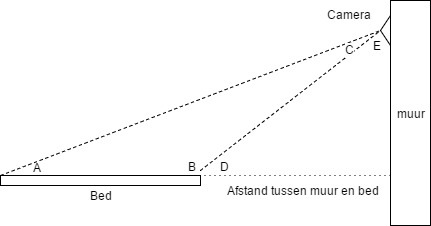
\includegraphics[scale=0.7]{CameraNietAanBed}
	\caption{Schets van camera niet bevestigd aan bed}
	\label{imgCNB}
\end{figure}
Net zoals bij de vorige berekening vindt u de namen van de hoeken terug in de afbeelding. Bij deze berekening nemen we aan dat de camera zelf geen dikte heeft. Dus de hoek E zit tussen de denkbeeldige lijn die de openingshoek van de camera weer geeft en de muur. Dit om de berekeningen iets eenvoudiger te houden. 
Over de hoeken hebben we volgende gegevens:
\begin{displaymath}
C=36^\circ
\end{displaymath}
\begin{displaymath}
A+B+C = 180^\circ
\end{displaymath}
\begin{displaymath}
B + D = 180^\circ \Rightarrow A = D-36^\circ
\end{displaymath}
Uit de sinus regel voor niet rechthoekige driehoeken kunnen we volgende formule afleiden:
\begin{displaymath}
\frac{2}{sin(36^\circ)}=\frac{s}{sin(D-36^\circ)}
\end{displaymath}
Door de cosinusregel in rechthoekige driehoeken, geldt volgende formule
\begin{displaymath}
cos(D)=\frac{x}{s}
\end{displaymath}
Uit de twee voorgaande formules kunnen we de waarde van D berekenen als we de waarde voor x kennen:
\begin{displaymath}
cos(D)sin(D-36 ^\circ)=\frac{x . sin(36^\circ)}{2}
\end{displaymath}
Vervolgens gaan we de tangens regel voor rechthoekige driehoeken gebruiken om h te bepalen:
\begin{displaymath}
h=tan(D) . x
\end{displaymath}
met:
\begin{description}
	\item [A, B, C, D, E] de hoeken zoals weergegeven in figuur \ref{imgCNRBB}
	\item[s] de schuine zijde in de driehoek (tussen B en C)
	\item[x] de afstand tussen het bed en de muur
	\item[h] de hoogte waarop de camera moet komen
\end{description}
Een overzicht van de berekende waarden, worden weergegeven in tabel \ref{refTabCNB}.

\begin{table}[hbp]
	\caption{Berekende waarden camera niet aan bed bevestigd}
	\begin{tabular}{|c|c|c|}
		\hline
		horizontaal & D & hoogte \\ \hline
		0.25 & 84 & 2.37 \\ \hline
		0.5 & 77 & 2.16 \\ 
		\hline
	\end{tabular}
	\label{refTabCNB}
\end{table}
Aangezien een kamer ongeveer 2,5 meter hoog is, zien we dat het mogelijk is de camera op een hoogte te plaatsten waardoor het volledige bed zichtbaar is.

\subsubsection{Besluiten bij de berekeningen}
Uit de eerste twee berekeningen besluiten we dat het onmogelijk is om de gebruikte camera aan het bed te bevestigen en heel het bed te zien. Er zijn twee mogelijke oplossingen. We kunnen een andere camera nemen met een grotere openingshoek, of we kunnen de camera verder van het bed plaatsen zodat de benodigde hoogte kleiner gaat worden.\\
Uit de tweede berekening kunnen we besluiten dat het met de gebruikte camera wel mogelijk is om het volledige bed in het frame te krijgen. Als we de camera achter het bed aan de muur hangen.

\section{Gebruikte technieken voor de gedragsanalyse}
\label{MRefMGA}
Deze sectie is opgebouwd uit twee verschillende delen. In het eerste deel bespreken we de dingen de we als eerste hebben gedaan in dit onderzoek, nog voor we begonnen zijn aan de effectieve gedragsanalyse. In het tweede deel bespreken we de gebruikte technieken aan de hand van de verschillende fasen in het werkingsschema, dat terug te vinden is in figuur \ref{imgWeS} en dat we hebben besproken in sectie \ref{MRefWeS}. Voor het maken van de gedragsanalyse en de code die we schrijven tijdens de voorbereidende technieken, wordt gebruik gemaakt van openCV, de gebruikte taal voor de code is c++. De code is terug te vinden op de cd die samen met deze tekst afgegeven is. 

\subsection{Voorbereidende technieken}
Voor we begonnen zijn aan de gedragsanalyse, hebben we eerst bekeken of we de camera met de gekregen code, aan de praat kregen op de computer. Vervolgens hebben we nagekeken of we met deze camera een persoon in een bed kunnen waarnemen. Nadien hebben we twee klassen geschreven. De eerst is SaveImage, deze heeft \'e\'en methode (saveImage) en heeft als doel het frame dat we ophalen met de gekregen code, weg te schrijven op het door ons gedefini\"eerde pad. De tweede geschreven klasse is de klasse GetImages. Deze heeft eveneens \'e\'en methode, namelijk getImage. Deze methode dat het frame op het door ons opgegeven pad weer ophalen. Deze technieken zijn gebruikt in het eerste experiment, meer informatie hierover is te vinden in sectie \ref{ERefOvB}. Tijdens deze fase van het onderzoek hebben we eveneens de camera op de juiste hoogte in de kamer gemonteerd zodat het bed volledig in het frame past. 

\paragraph{Opmerkingen}
openCV beschikt over standaardfunctie voor het wegschrijven en ophalen van afbeeldingen. Wij gebruiken deze, maar hebben de twee klassen geschreven omdat er voor het opslaan van de afbeelding een conversie moet gebeuren om de afbeeldingen om te zetten naar het juiste bestandstype. Anders zouden we de conversie elke keer apart moeten oproepen. Het bespaart elke keer een paar lijnen code en we verkleinen eveneens de kans dat iemand het vergeet of er een fout in getypt worden.\\
Nadat deze fase afgelopen was, hebben we de Klassen SaveImages en GetImages samengevoegd tot \'e\'en klasse, namelijk SGImage. De twee methodes worden vervolgens voor deze klasse ge\"implementeerd. Dit omdat we nu nog maar \'e\'en object moeten aanmaken om zowel afbeeldingen op te slaan als terug op te halen. Dit is effici\"enter. \\
Het opslaan en ophalen van de afbeeldingen is ook nodig voor het maken van opeenvolgende tesbeelden. Zo kunnen we overdag de ontwikkelde technieken laten lopen over dezelfde beelden en hier besluiten uit trekken. Verder maakt dit dat we ook niet elke keer als we iets willen testen we een persoon moeten zoeken die dan even in een bed wilt gaan liggen.

\subsection{Ontwikkelen van de gedragsanalyse}
\label{mRefOGA}
Zoals eerder aangehaald, gaan we de gebruikte methodes van dit deel van het onderzoek overlopen aan de hand van het werkingsschema. Dit is terug te vinden in afbeelding \ref{imgWeS}. De gebruikte technieken zijn terug te vinden in de volgende paragrafen.

\subsubsection{Persoon in bed}
\begin{figure}[hbp]
	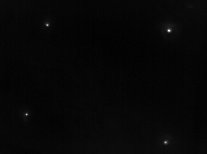
\includegraphics[scale=0.75]{SeekCamBed}
	\caption{Foto van het bed met warme objecten op de hoeken}
	\label{imgCBe}
\end{figure}
Het eerste blokje in het werksschema is persoon in bed. We hebben een klasse Bed gemaakt. Een object van de klasse bed bestaat uit acht integers. Dit zijn de co\"ordinaten van de hoekpunten van het bed. Dankzij deze kunnen we achteraf bepalen of een persoon in bed ligt, of aanstalten maakt om eruit te komen. Verder hebben we in dit stadium ook een mousecallback functie gemaakt deze wordt besproken in de eerstvolgende paragraaf, daarna volgt een bespreking van de Bed klasse \\

\paragraph{mouseCallBack functie}
 De functie gaat de punten waarop geklikt wordt, met de linkermuisknop opslaan in een vector. Door een klik met de rechtermuisknop, wordt het laatste punt in de vector verwijdert. Door op enter te klikken wordt de functie be\"eindigd. 
 
\paragraph{klasse Bed}
De klasse bezit drie costructoren. De eerste heeft geen argumenten. Indien deze opgeroepen wordt is het bed object een punt. De tweede constructor, heeft acht integers als argument. Deze methode heeft een paar nadelen. Je moet de hoekpunten van het bed op voorhand kennen. Deze zijn moeilijk om te berekenen. Om het voor de gebruikers van het systeem gemakkelijker te maken hebben we een andere constructor ontwikkeld.  De derde constructor heeft twee argumenten. Het eerste is een afbeelding en het tweede is een integer. De afbeelding is een frame waarop een leeg bed te zien is, waar op elke hoek van het bed een warm object geplaatst is. Een voorbeeld van zo een afbeelding is te zien in figuur \ref{imgCBe}. De camera gaat de warme objecten weergeven als lichte punten op een donkere achtergrond. Het tweede argument, de integer gaat bepalen op welke manier de co\"ordinaten van de lichtere punten in de afbeelding toegekend worden aan de integers van het bed object. Als de integer 0 is, dan wordt er via de mouseCallBack functie, die eerder is besproken, gevraagd om de hoekpunten van het bed aan te klikken, beginnend bij het hoekpunt rechtsboven. Op elk punt moet dan \'e\'en keer geklikt worden. De klik positie wordt toekend aan het bed object. Als de integer van het argument een andere waarde heeft als 0. Dan worden de locaties van de punten via blobdetectie automatisch uit de afbeelding opgehaald en toegekend. Deze constructor is veel gebruiksvriendelijker. Er moet wel eerst een afbeelding van het bed beschikbaar zijn. Deze kan eenvoudig gemaakt worden door het programma saveBed te gebruiken. saveBed gaat \'e\'en frame ophalen en dit opslagen in het mapje van bed. Daar kan deze achteraf makkelijk opgehaald worden.\\
\begin{figure}[hbp]
	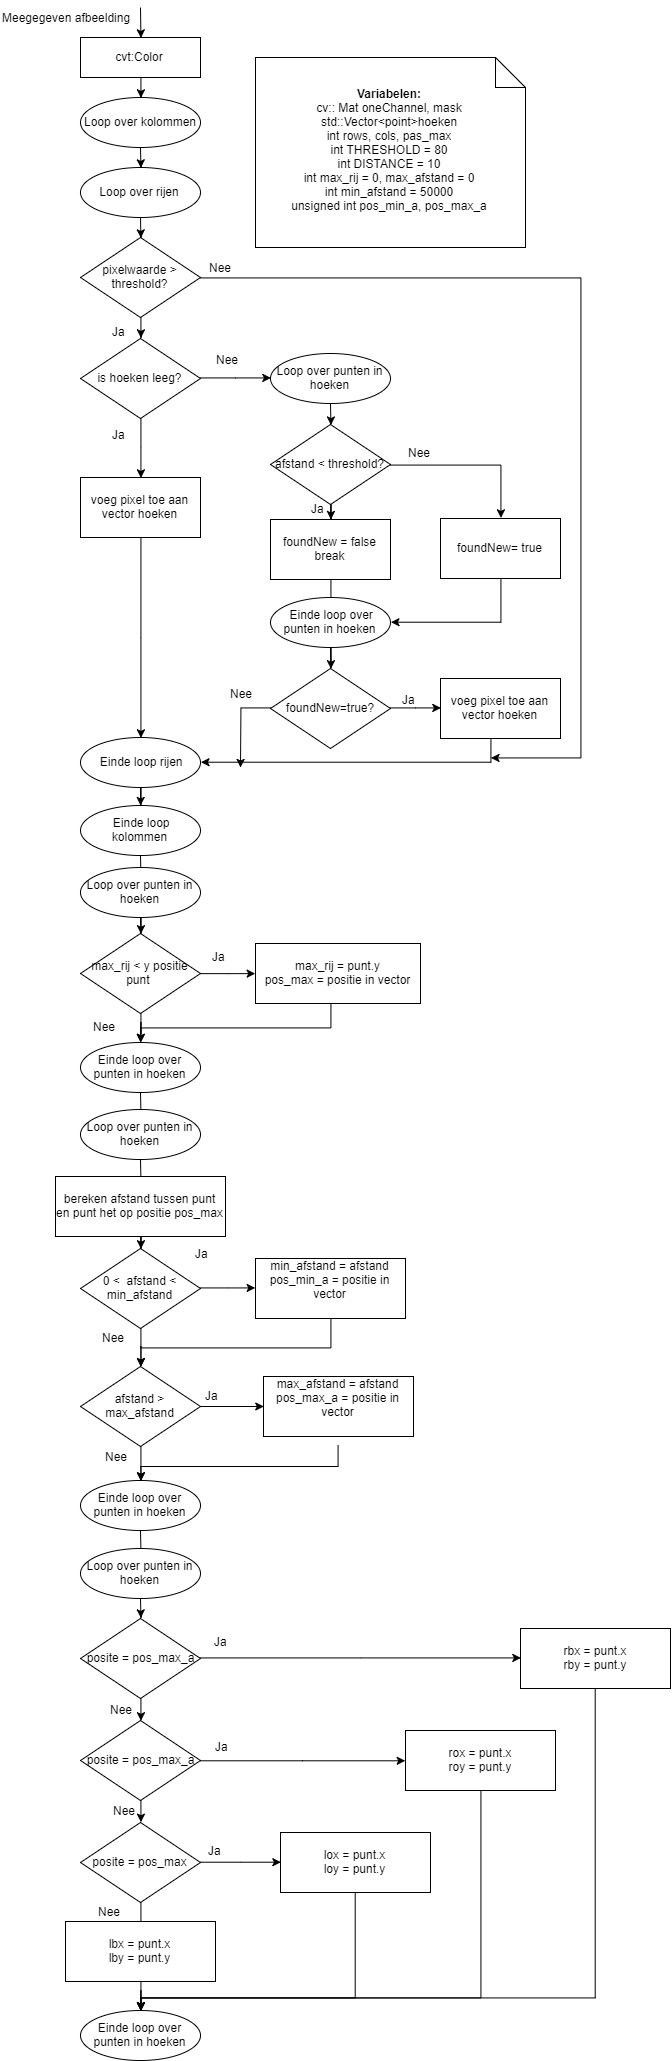
\includegraphics[scale=0.34]{FlowChart_setValuesAuto}
	\caption{Flowchart van de methode setValuesAuto}
	\label{imgFCSVA}
\end{figure}
De klasse bed heeft een aantal andere methodes, de eerste is setValues deze heeft acht integers als argument en gaat deze toekennen aan de integers van het object. Een andere methode is seValuesImg, deze gaat via de mouseCallBack functie de waarden van de co\"ordinaten toekennen aan het object. setValuesAuto gaat automatisch de hoekpunten bepalen aan de hand van de weergegeven afbeelding. de flowchart van deze methode is te zien in figuur \ref{imgFCSVA}. De methode werkt als volgt, er wordt een lege vector gecre\"erd. Vervolgens lopen we over alle pixels in de afbeelding, als de pixel licht is, wordt er gezien of we de waarde aan de vector moeten toevoegen. De pixelwaarde moet toegevoegd worden als de vector nog leeg is, of als er geen punt in de directe omgeving in de vector staat. Als we door alle pixels hebben gelopen, gaan we bepalen welk punt het meest onderaan staat. Dit is de linker onder hoek. Door gebruikt te maken van de onderlinge afstand van dit punt met de drie andere punten in de vector, worden de waarden aan de juiste hoeken toegekend. Een andere methode is sidesOfBed. Deze methode gaat aan de hand van de hoeken van het object, de zijkanten van het bed bepalen. Dit zijn twee vergelijkingen van rechten. De co\"effici\"enten van deze vergelijkingen worden in een vector terug gegeven. De laatste methode van Bed, is de headOfBed. Deze gaat aan de hand van de hoekpunten de vergelijking van een lijn bepalen. Als de persoon in het bed ligt, gaat het hoofd boven de lijn liggen. De laatste twee methodes worden gebruikt tijdens de detectie van de persoon in het bed of het uit het bed stappen.


\subsection{Persoon in bed?}
\label{mrefPIB}
Persoon in bed? is de tweede blok van het werkingsschema. Dit is het deel van de gedragsanalyse waar het meeste tijd in kruipt. Er zijn veel verschillende versies gebruikt om de detectie van een persoon te doen. Deze technieken zijn methodes van een nieuwe klasse. Deze klasse is de klasse Detect. De klasse Detect is opgebouwd uit een Bed object. De klasse Detect heeft twee contstructoren. De eerst heeft acht integers als argument. Als deze opgeroepen wordt, wordt er een punt bed object gecre\"erd, nadien worden met de setValues methode van de klasse bed de co\"ordninaten van de hoekpunten toegekend. De tweede constructor heeft een afbeelding als argument, na de creatie van het punt object, wordt door gebruik te maken van de methode setValuesAuto van de klasse bed de hoekpunten toegekend. In de volgende paragrafen bespreken we methodes die in deze klasse gemaakt zijn en gebruikt worden om de persoon in het bed te detecteren.

\subsubsection{Eerste poging: createMask}
\begin{figure}[hbp]
	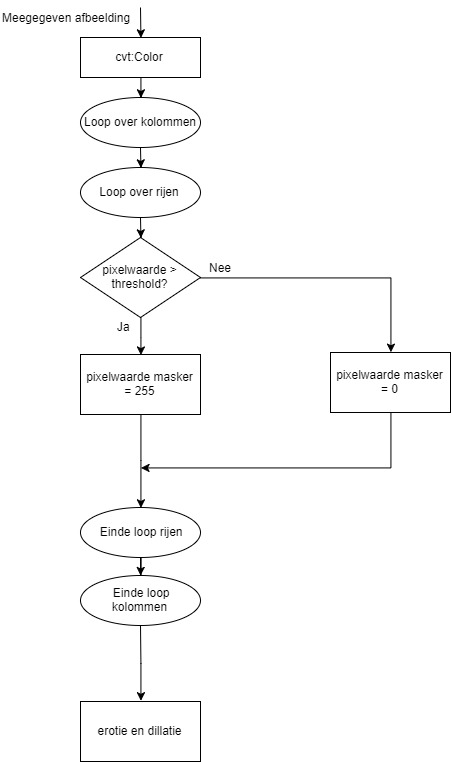
\includegraphics[scale=0.6]{FlowChart_createMask}
	\caption{Flowchart van de methode createMask}
	\label{imgFSCMa}
\end{figure}
Deze methode is gebaseerd op het thresholden van kleuren. Deze techniek is besproken in de literatuurstudie in sectie \label{refTVK}. Aangezien wij een grijswaarden afbeelding hebben, hebben we maar \'e\'en threshold waarmee vergeleken moet wordt. De flowchart van deze methode wordt weergegeven in figuur \ref{imgFSCMa}. De gekozen threshold is 180. Deze waarde is bekomen door middel van het princiepe van trial and error. Na afloop wordt erosie en dilatie toegepast. Hiermee gaan we de ruis verminderen. Figuur \ref{imgCMa} geeft een frame en het verkregen masker weer. We zien dat het masker het gewenste resultaat vertoont.
\begin{figure}[hbp]
	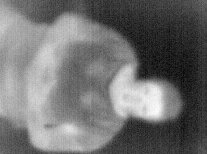
\includegraphics[scale=0.75]{EersteExperiment_img0}
	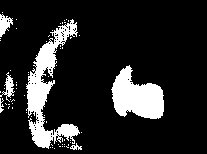
\includegraphics[scale = 0.75]{EersteExperiment_mask0}
	\caption{Voorbeeld van masker: (links) meegegeven afbeelding (rechts) verkregen masker}
	\label{imgCMa}
\end{figure}
\paragraph{Opmerkingen}
Doordat de het bed opgewarmd wordt door de lichaamswarmte. Wordt de restwarmte, dit is de warmte die achterblijft in het bed nadat de persoon eruit gestapt is, ook gedetecteerd als een persoon. Een afbeelding hiervan wordt getoond in figuur \ref{imgCOB}. Verder worden er ook nog andere warme plekken gedetecteerd, die geen deel uitmaken van een persoon. Door deze valse persoon detecties hebben we een tweede manier van detectie gecre\"eerd. Deze wordt besproken in de volgende paragraaf.

\subsubsection{Tweede poging: temporeel verschil}
\begin{figure}[hbp]
	\includegraphics[scale=0.6]{FlowChart_TempDifference}
	\caption{Flowchart van de methode tempDifference}
	\label{imgFCTDi}
\end{figure}
Om het probleem van de restwarmte op te lossen, hebben we het temporeel verschil ge\"introduceert. Deze techniek is in de literatuurstudie besproken in sectie \label{refBET}. De gedacht hier is eerst te gaan zien waar er beweging is, dit is waar de pixelwaard voor twee opeenvolgende frames niet gelijk is. Dit wordt gedaan door de methode tempDifference van de klasse Detect. Om de werking hiervan te verduidelijken is de flowchart toegevoegd.  Deze is te zien in figuur \ref{imgFCTDi}. Het resultaat van deze methode noemen we vanaf nu het bewegingsmasker. Een voorbeeld van een bewegingsmasker is weergegeven in figuur \ref{imgBMa}.
\begin{figure}[hbp]
	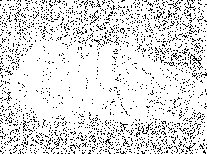
\includegraphics[scale=0.75]{bewegingsMatrix}
	\caption{Voorbeeld van een bewegingsmasker}
	\label{imgBMa}
\end{figure}
We zien dat er veel pixels wit zijn in zo een bewegingsmasker. Dit komt doordat alle pixels die kouder worden, zoals bijvoorbeeld een deel van het bed dat afkoelt nadat een persoon hier gelegen heeft, ook mee gedetecteerd worden. Verder is een verandering van pixelwaarde met 1 ook voldoende om gedetecteerd te worden. Omdat er toch veel niet interessante regio's gedetecteerd worden. Hebben we de methode createMask aangepast. Deze heeft nu twee argumenten het bewegingsmasker en het huidige frame. De functie gaat nu een masker cre\"eren waarbij witte pixels voorkomen op de plaatsen waar de pixelwaarde in het huidige frame boven de threshold waarde is en de overeenkomende pixelwaarde van het bewegingsmasker ook wit is. De werking van deze methode wordt verduidelijkt aan de hand van een flowchart, weergegeven in figuur \ref{imgFCCMN} geeft een masker bepaald door de creatMaskNew methode en het huidige frame weer.
\begin{figure}[hbp]
	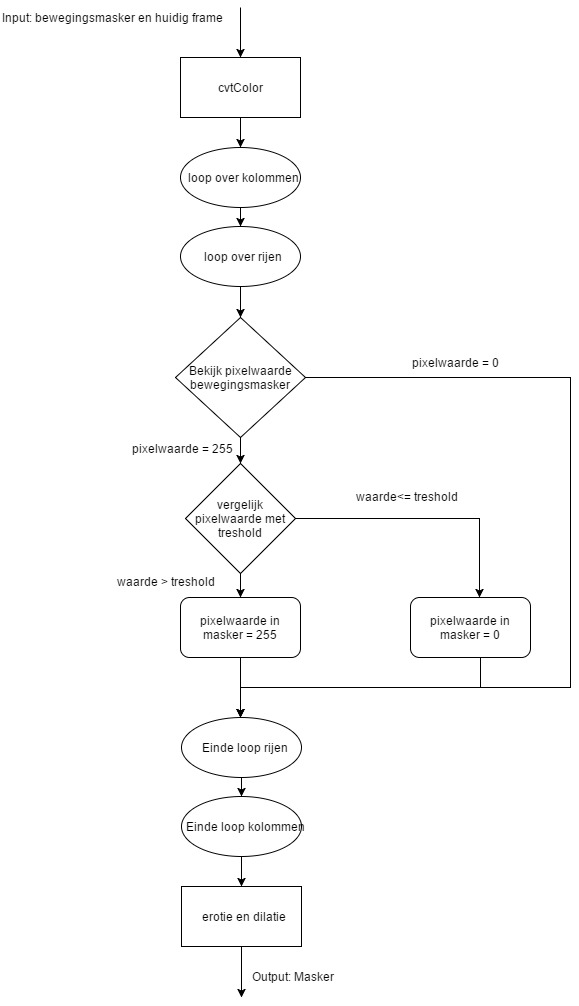
\includegraphics[scale=0.6]{FlowChart_createMaskNew}
	\caption{Flowchart van de methode createMaskNew}
	\label{imgFCCMN}
\end{figure}
Figuur \ref{imgCMN}
\begin{figure}[hbp]
	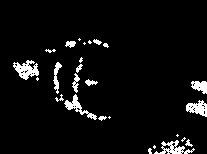
\includegraphics[scale=0.65]{MaskMetDif}
	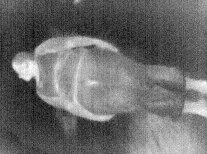
\includegraphics[scale=0.65]{ImgMetDif}
	\caption{Frame en masker gemaakt met methode createMaskNew}
	\label{imgCMN}
\end{figure} 
Er worden nog steeds punten gedetecteerd die voor ons niet van toepassing zijn. Verder is er ook nog veel restwarmte die tot valse persoonsdetecties kan leiden.


\subsubsection{Derde poging: aangepast temporeel verschil}
De twee voorgaande algoritmes hebben gefaald door het restwarmte probleem. Dit algoritme heeft als doel daar iets aan te doen. We hebben de methode tempDiffNew aangepast. Vanaf nu krijgt het bewegingsmasker de waarde 255 als de pixelwaarde van het nieuwe frame hoger is dan de pixelwaarde van het vorige frame. Als de persoon uit het bed stapt is dit bed nog warm, dit is dus restwarmte. Dit gaat in de komende tijd afkoelen tot kamertemperatuur. Daardoor zou dit niet meer gedetecteerd mogen worden in deze nieuwe methode. Verder wordt het algoritme op de zelfde manier opgebouwd als in de voorgaande poging. In sectie \ref{ERefRVB} zijn een paar van deze maskers te zien en worden de resultaten besproken. Dit was dus niet het gewenste resultaat. Dit probleem en het feit dat de restwarmte lang aansleept komt door de normalisatie van de pixelwaarden. Daarom hebben we dit algoritme ook toegepast op beelden voor de normalisatie optreedt. Buiten het weglaten van de normalisatie stap is het gehele algoritme behouden. Dit geeft geen goede resultaten omdat de camera een bereik van -40 tot 330 $^\circ$c heeft. Het verschil tussen kamer temperatuur rond de 20 $^\circ$c en de lichaamstemperatuur van 37 $^\circ$c is niet groot genoeg om via threshold te detecteren. Op deze manier kunnen we geen correcte persoonsdetectie doen. 

\subsubsection{Vierde poging: detectie van het hoofd}
Als laatste algoritme voor de detectie van persoon in bed, werken we alleen met het hoofd. Dit is altijd zichtbaar, ook als een persoon onder een deken slaapt. Verder wordt dit ook niet bedekt door kleding. De methode die we hier gebruiken is detectionHead, er wordt een masker meegegeven. Het masker is een gewoon masker gecre\"eerd met createMask. We gaan zien of het hoofd zich bevind het hoofdgedeelte van het bed. Het hoofdgedeelte van het bed wordt bepaald door de methode headOfBed van de klasse Bed. Praktisch doen we dit door een vorm van blobdetectie. We gaan over alle pixels van het masker lopen. Als een witte pixel gevonden wordt, gaan we indien de resultaten vector leeg is, de waarde in de vector opslaan. Indien de resultaten vector niet leeg is, gaan we zien of er al een punt uit de omgeving in de vector zit. Indien er al een punt uit de omgeving in de vector zit, worden de co\"ordinaten van dit punt mee in de berekening het gemiddelde punt genomen. We vergelijken de gevonden punten met deze gemiddelde waarde bij het toevoegen in de vector. Indien er geen gemiddelde waarde in de omgeving van het punt ligt, wordt er een nieuw punt toegevoegd aan de vector.  Nadat alle pixels doorlopen zijn, gaan we over de gemiddelde punten lopen in de vector. We vergelijken de positie van deze punten met de lijn die het hoofdeinde scheidt van de rest van het bed. Als er een hoofd in de juiste regio gevonden wordt, wordt er true terug gegeven, anders false.

\subsection{links naast bed?}
Indien we de persoonsdetectie doen aan de hand van het hoofd, gaan we de detectie van naast het bed doen als er false terug gegeven wordt na uitvoering van de methode detectionHead. We gaan dan het masker meegeven met de functie checkBed uit de klasse Detect.\\
Voor de andere algoritmes die besproken zijn in sectie\ref{mRefPIB}, gaan we  de verkregen maskers of bewegingsmaskers uit de vorige sectie , worden meegegeven met de methode checkBed uit de klasse Detect.\\
Het doel van deze methode is gaan kijken of er witte delen van het masker zich buiten het bed bevinden. Deze methode heeft \'e\'en argument. Dit is het masker. We gaan over alle pixels lopen. Als de pixel van het masker wit is, gaan we kijken waar dit punt ligt ten opzichte van de zijkanten van het bed. De zijkanten worden bepaald door de methode sidesOfBed van de Bed klasse. Er wordt weergegeven langs welke zijde het witte deel zich bevindt. Als er geen witte delen buiten het bed zijn, dan wordt None terug gegeven.
\paragraph{Opmerkingen}
De methode checkBed kan eventueel ook ge\"optimaliseerd worden. In plaats van over alle pixels te lopen en te zien of het masker daar een waarde van 255 heeft, kan men ook enkel over de pixels lopen die geen deel uitmaken van het bed.

\subsection{Timer}
We hebben voor het bijhouden van hoelang de persoon uit het bed is, een nieuwe klasse Alarm gedefinieerd. Deze timer bevat een teller en een threshold. Deze klasse heeft \'e\'en constructor, deze wordt opgeroepen als er voor de eerste keer geen persoon in bed gedetecteerd wordt. Deze zet de teller op 0. Als in het volgende frame geen persoon aanwezig is, dan wordt de methode adOne opgeroepen. Deze gaat de teller incrementeren. Vervolgens gaat hij de teller met de threshold vergelijken. Als de teller groter of gelijk is aan  de threshold, dan wordt via de methode timesUp een alarm gegenereerd. Als de persoon terug in bed is of er is iemand van de verpleging langs geweest, dan wordt via endAlarm het alarm gestopt. Er is nog \'e\'en overige methode. Via setThresh kan je de threshold instellen indien de standaardwaarde niet goed is voor de desbetreffende kamer. 

\section{Overige methodes}
\label{MrefOvM}
\subsection{checkMovement}
Deze methode gaat 2 opeenvolgende frames vergelijken om te zien of het de moeite is om de volgende zwaardere berekeningen te doen. Indien er geen beweging is geweest, kan de persoon ook niet uit bed gestapt zijn, of eruit gevallen. Deze methode heeft als argument 2 opeenvolgende frames. Deze worden pixel per pixel vergeleken. Het aantal pixels waar er een verschillende waarde is wordt bijgehouden. Deze wordt vergeleken met een drempelwaarde. Indien het aantal verschillende pixels kleiner is dan de drempelwaarde, is er geen beweging geweest en wordt false terug gegeven. Indien er wel meer verschillende pixelwaarden zijn, heeft de persoon bewogen en wordt er true terug gegeven.

\subsubsection{erDil}
Deze methode heeft twee argumenten. De eerste is de afbeelding waarop de erosie en dilatie toegepast moet worden. Het tweede is de grootte van de matrix gebruikt voor het eroderen en dileren. Hoe groter de waarde, hoe meer details er van de afbeelding verdwijnen. Nadat de erosie en dilatie, wat men ook wel openen noemt, is toegepast wordt de resultaatafbeelding terug gegeven. Deze methode wordt tijden het maken van een masker opgeroepen. 

\section{Besluit over de methode}
\label{MRefBes}
Tijdens ons onderzoek maken we gebruik van een infraroodcamera. Er zijn echter nog andere types van camera mogelijk. Hiernaar hebben we geen onderzoek gedaan. Een mogelijk uitbereiding van dit onderzoek is om onze gedragsanalyse mits een paar aanpassingen, te gebruiken op beelden gemaakt met een andere type camera.
Verder kunnen we besluiten dat er veel verschillende methodes van persoonsdetectie mogelijk zijn. Deze gaan echter niet allemaal tot een goed resultaat leiden. Verder zijn er een paar methodes waar er optimalisatie mogelijk is. Zoals bijvoorbeeld de checkBed methode. We hebben onze methode gebaseerd op het werkingsschema weergegeven in figuur \ref{imgWeS}. We kunnen dus besluiten dat het mogelijk is om een analyse volgens dit schema op te bouwen. Een andere mogelijke uitbereiding is het toevoegen van valdetectie. In hoofdstuk \ref{ERef} worden de verschillende experimenten besproken.